\documentclass{IEEEtran}
\usepackage{graphicx}
\usepackage{blindtext}
\usepackage{float}
\usepackage{amsmath, amssymb}
\usepackage{url}

\begin{document}

  \title{Time Series Analysis and Distribution Fitting of Wind Speed and Wind Power Data}
  \author{\IEEEauthorblockN{Adam Carrera}
  \IEEEauthorblockA{\\Erik Jonsson School of Engineering \\
  The University of Texas at Dallas \\
  email: anc170430@utdallas.edu}}

  \maketitle

  \begin{abstract}
    A time series analysis of wind speed and wind power data is preformed. Distributions are fitted to the wind speed and wind power data. The wind speeds are fitted with three different types of distributions and evaluated based on the KS test. The wind power is fitted with a Gaussian Mixture Model. Different numbers of clusters along with covariance matrix formulation are tested and evaluated using the Bayesian Information Criterion.
  \end{abstract}

  \section{Introduction}

  From 2008 to 2012 wind data was collected at Site A. The data contains variables such as wind speed, wind power, wind direction, air temperature, surface air pressure, and density at hub height. Data was collected once every 5 minutes for the entire year. In this paper we are going to analyze the wind speed and wind power by looking at the time series data and the probability distributions.

  \section{Time Series Analysis}

  Before we take a look at any distributions or distribution fits, we must first plot and visualize the data. By doing this we are able to visualize patterns, changes over time, and observe anything unusual. Additionally, we can analyze how the wind speed changes seasonally. First we will plot the time series of the wind speed.

  \subsection{Time Series}

  A time series can be thought of as a list of numbers, along with some information about what times those numbers were recorded \cite{forecasting}. For our purposes, the wind speed is our time series. The wind speed was measured once every 5 minutes at Site A for one five years, from 2008 to 2012.

  \subsection{Wind Speed Time Series}

  Fig. \ref{fig:seasonal1} shows a time series seasonal plot for the wind speed of the first week in each year. We can notice some trends, generally, the wind speed seems to drop sharply at the beginning of the week, rise sharply, and decrease gradually throughout the rest of the week. Additionally, we can see that the wind speed does not increase for each year. Finally, we can notice some cyclic fluctuations for each year.

  \begin{figure}[ht!]
    \centering
    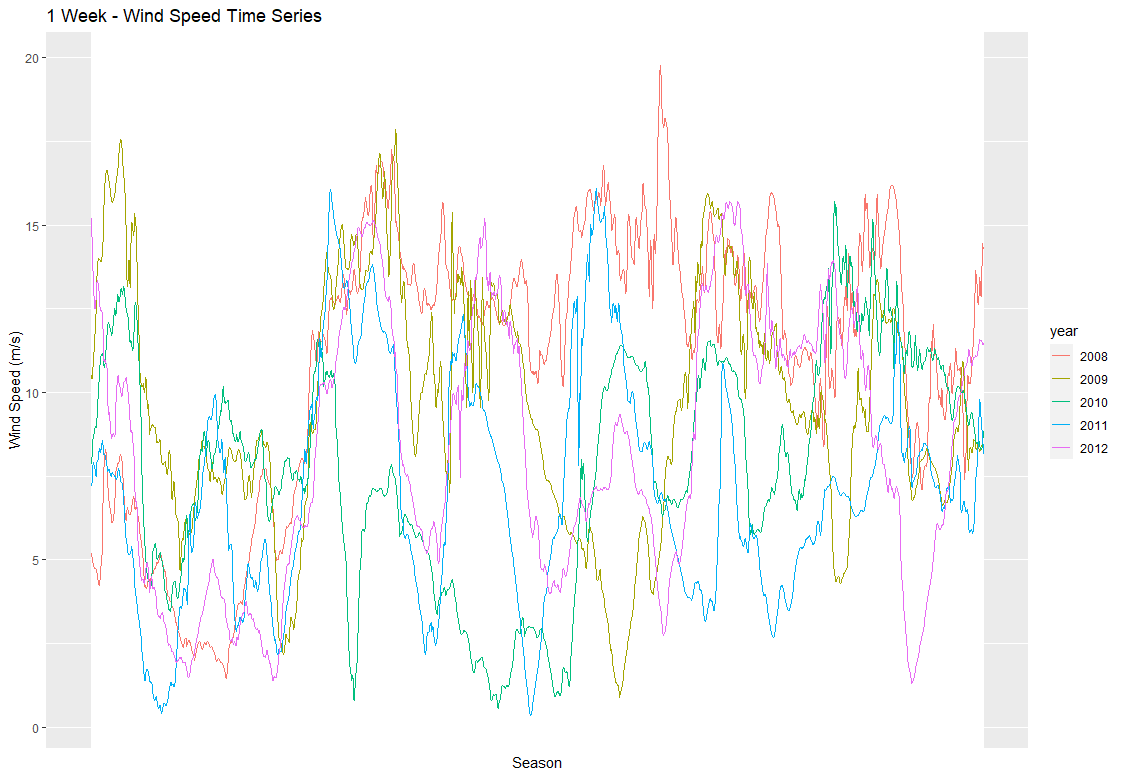
\includegraphics[width=0.45\textwidth]{figures/seasonalweek}
    \caption{Seasonal Plot of Wind Speed Time Series - the first week of 2008 through 2012}
    \label{fig:seasonal1}
  \end{figure}

  The weeklong analysis is a subset of a larger picture. The windspeed seasonal plot for the entire year is too complex to visually analyze so we will be smoothing the data with a 30 day moving average. Fig. \ref{fig:seasonal2} shows the year long seasonal plot. We can observe some much larger trends. Towards the end of the year the windspeed drops steadily, and then rises again.

  \begin{figure}
    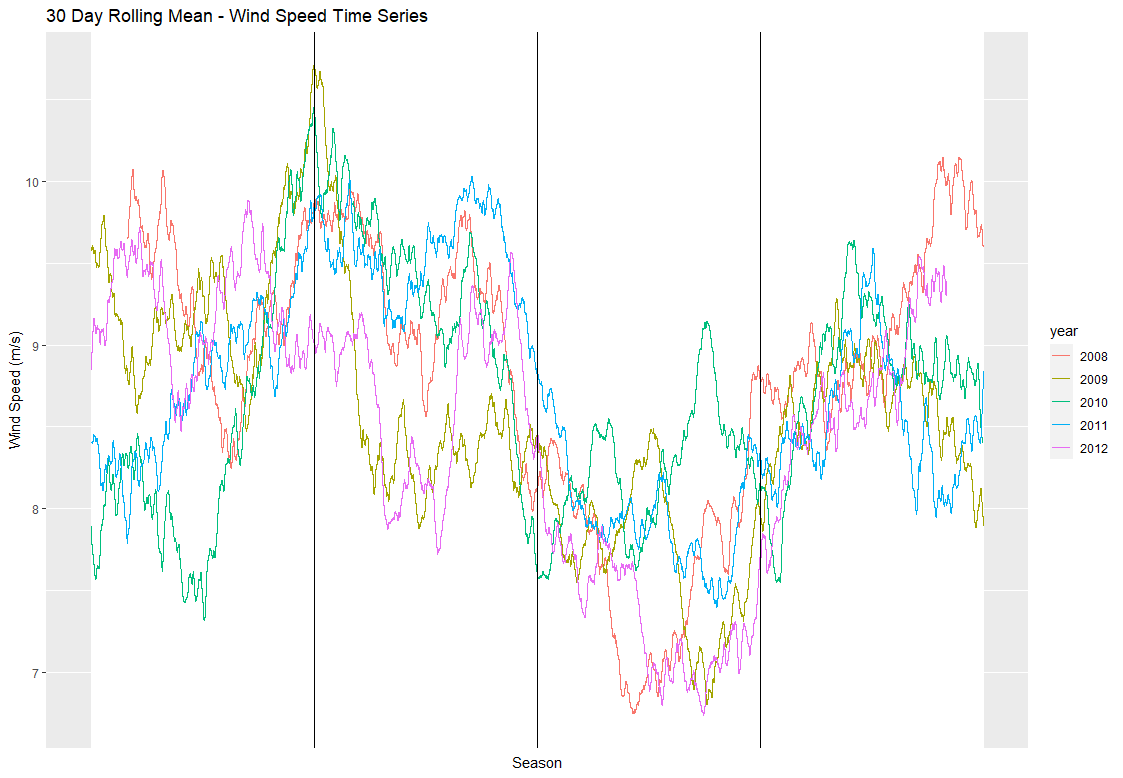
\includegraphics[width=0.45\textwidth]{figures/seasonalyear}
    \caption{Seasonal Plot of Wind Speed Time Series - 2008 through 2012. The x-axis divides the year into four seasons.}
    \label{fig:seasonal2}
  \end{figure}

  \subsubsection{Moving Average}

  In statistics, a moving average is a calculation to analyze data points by creating a series of averages of different subsets of the full data set \cite{average}. A moving average is commonly used with time series data to smooth out short-term fluctuations and highlight longer term trends or cycles \cite{average}.

  \subsection{Wind Power Time Series}

  Fig. \ref{fig:seasonal3} shows a time series seasonal plot for the wind power of the first week in each year. We can see that the plant can generate a maximum of 2 MW which tends to fluctuate every now and then. We can also see that there are time periods where the plant is not generating any power at all. In Fig. \ref{fig:seasonal4}, we can see the 30 day moving average of the wind power, which behaves similarly to the 30 day moving average of the wind speed.

  \begin{figure}[ht]
    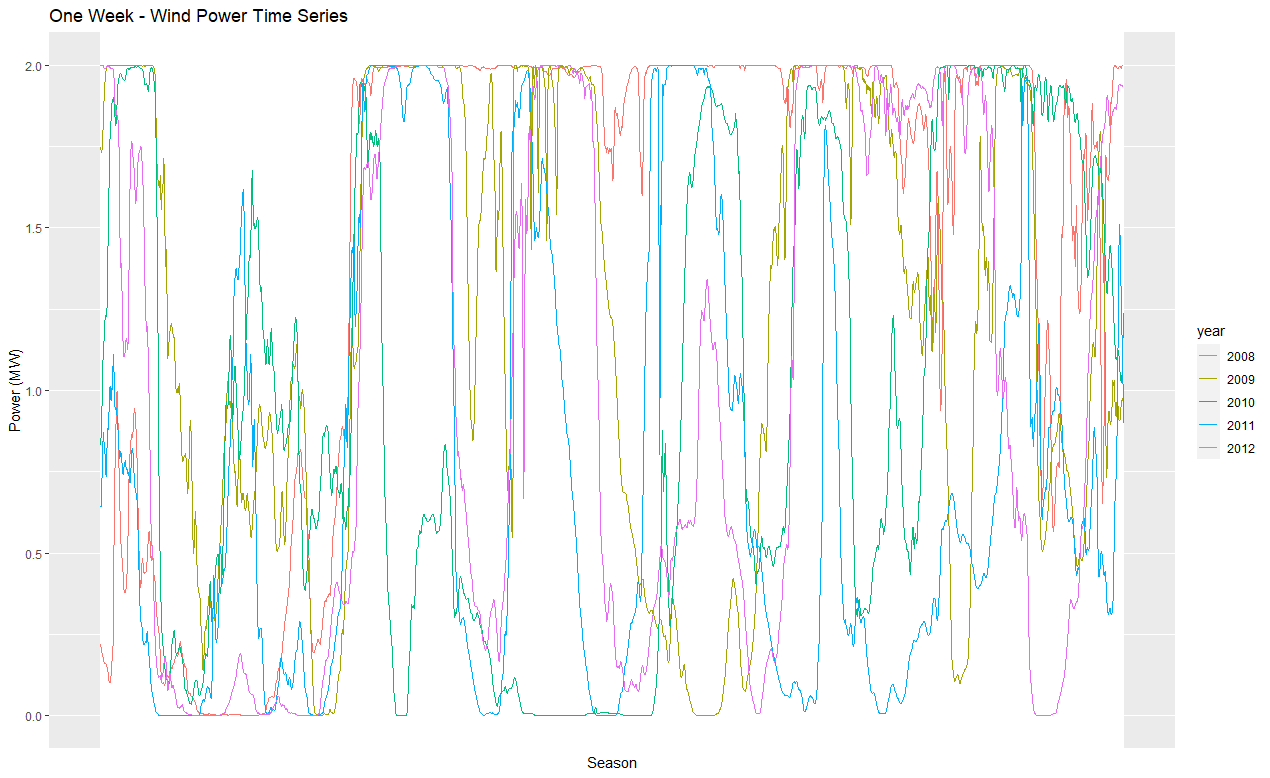
\includegraphics[width=0.45\textwidth]{figures/weekpower}
    \caption{Seasonal Plot of Wind Power Time Series - the first week of 2008 through 2012}
    \label{fig:seasonal3}
  \end{figure}

  \begin{figure}
    \centering
    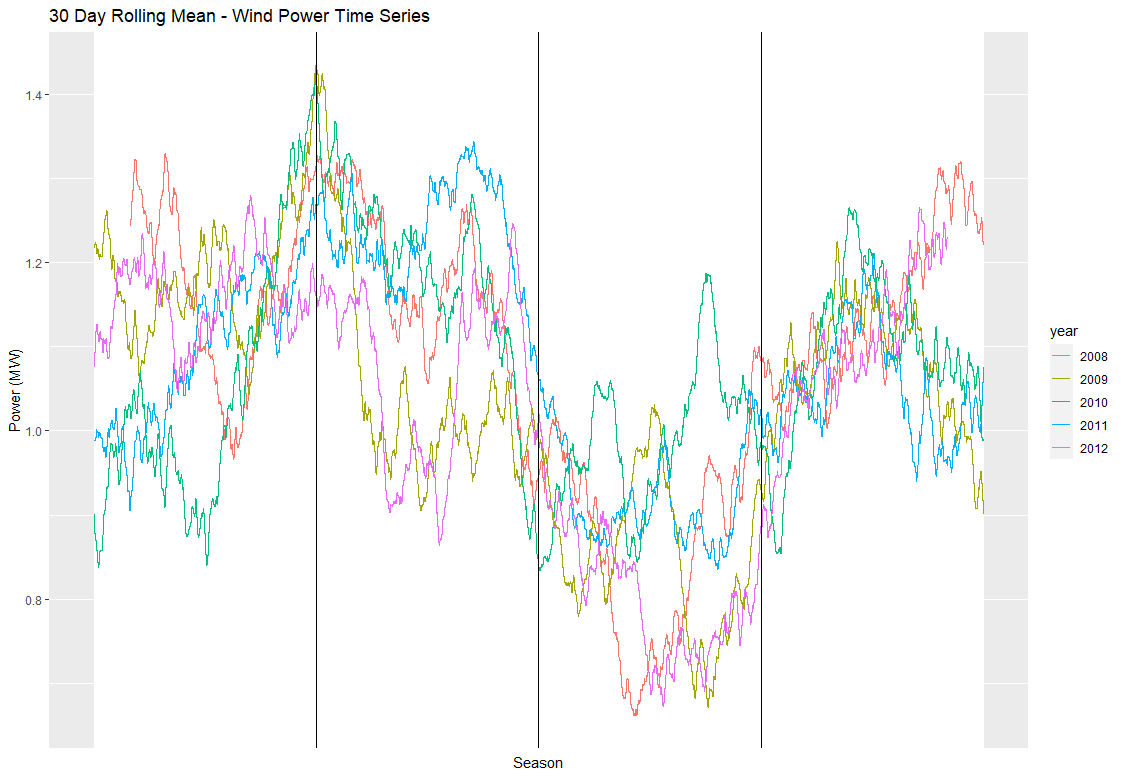
\includegraphics[width=0.45\textwidth]{figures/yearpower}
    \caption{Seasonal Plot of Wind Power Time Series - 30 Day Rolling Average - 2008 through 2012. The x-axis divides the year into four seasons.}
    \label{fig:seasonal4}
  \end{figure}

  \subsection{The Effect of Wind Speed on Wind Power}

  Clearly, wind speed and wind power are related. When we compare Fig. \ref{fig:seasonal1} to Fig. \ref{fig:seasonal3} we can see that the site will not generate any power if the wind speed falls below a certain value. Additionally, the wind speed only needs to be at a value of about 12 m/s for the site to generate at its full potential. Comparing Fig. \ref{fig:seasonal2} to Fig. \ref{fig:seasonal4} shows that the wind power and wind speed follow similar seasonal trends. For example, mean power generation falls steadily towards the end of the year along with wind speed, suggesting the two are correlated. Figure \ref{fig:comparison} shows the wind speed plotted against wind power for one week in each year from 2008 to 2012. We can see that the two values are correlated along with the minimum wind speed required to generate power (about 3 m/s) and the wind power required for maximum power generation.

  \begin{figure*}
    \centering
    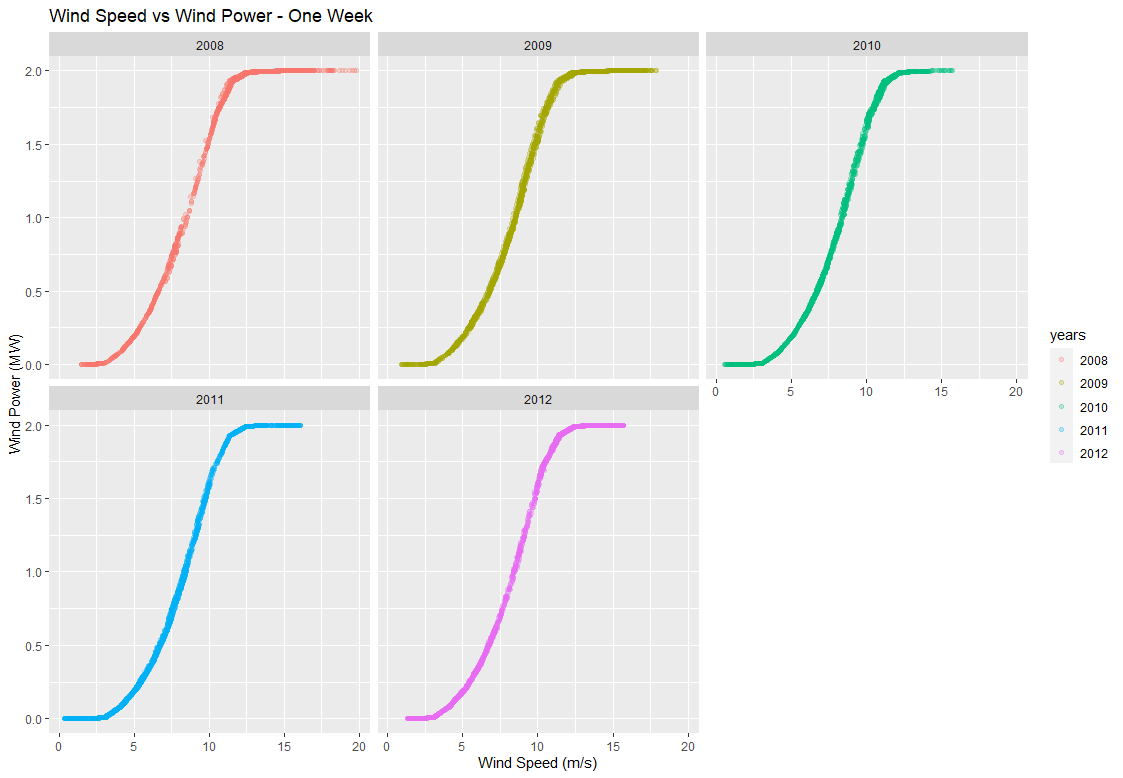
\includegraphics[width=0.75\textwidth]{figures/correlation}
    \caption{Wind Speed versus Wind Power for one week in 2008 through 2012 - this shows the relationship between wind speed and wind power, along with the minimum wind speed required to generate power, and the maximum wind speed required for full power generation}
    \label{fig:comparison}
  \end{figure*}



  \section{Wind Speed Distribution Analysis}

  A Probability Density Function (PDF) shows the probability of a certain value. In our application, we will see empirical PDFs for wind speed and wind power over several years. These distributions will show how likely it is for the wind to be at a certain speed, or for the wind farm to generate a certain power. Later in this paper, we will be fitting theoretical PDFs to our data. This will allow us to make forecasts and predictions regarding wind speed and wind power.

  \subsection{Empirical PDF - 2008 through 2012}

  Fig. \ref{fig:dist1} shows the wind speed density for the years 2008 through 2012. We can see that the most likely values in this time period were a little less than 10 m/s. Fig. \ref{fig:pwr1} shows the empirical PDF for wind power. We can see that this wind power PDF looks a lot different than the wind speed PDF. The most likely values for wind power were either 0 MW or 2 MW. Values of 0 MW may indicate low wind speeds, or the power plant not operating. Values of 2 MW indicate the power plant is operating and generating electricity. Because 2 MW is the highest and most common value, we can infer that the power plant is designed to output 2 MW constantly and every now and then we will see a slight fluctuation.

  \begin{figure}[hbt!]
    \centering
    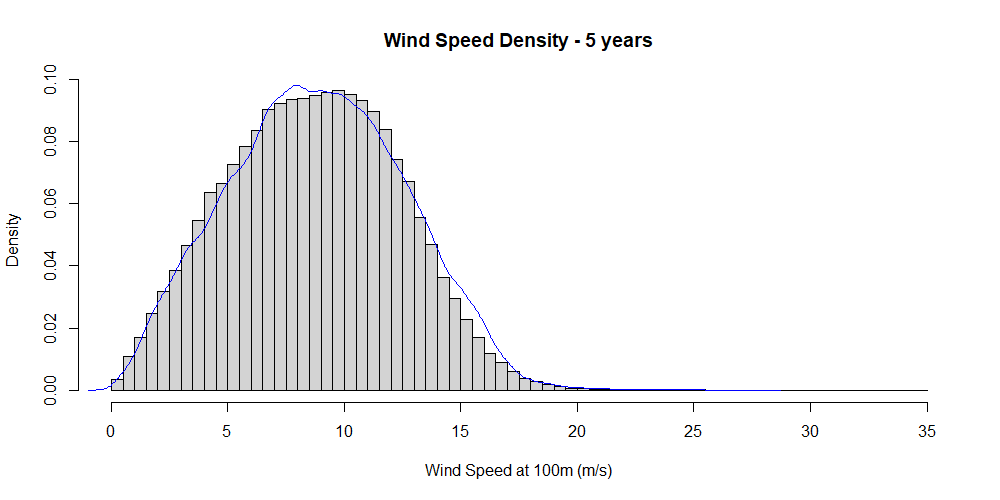
\includegraphics[width=0.45\textwidth]{figures/speeddensity5years}
    \caption{Wind Speed Density - 2008 to 2012}
    \label{fig:dist1}
  \end{figure}

  \begin{figure}
    \centering
    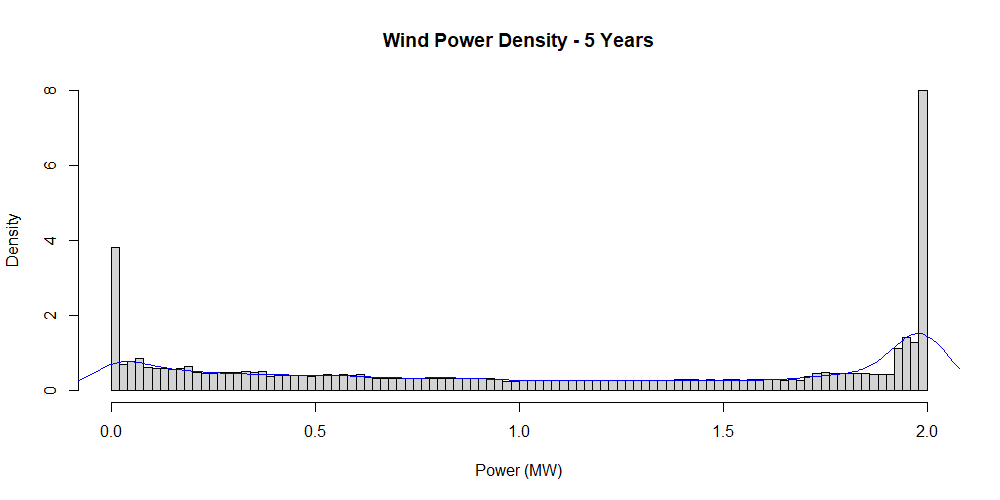
\includegraphics[width=0.45\textwidth]{figures/powerdensity5years}
    \caption{Wind Power Density - 2008 to 2012}
    \label{fig:pwr1}
  \end{figure}

  \subsection{Empirical PDF - Individual Years}

  Visually, the PDF plots for each individual year are very similar. The key differences lie in there mean and standard deviation values. Table \ref{tab:tab2} shows the $ \mu \text{ and } \sigma $ values for the wind speed from 2008 to 2012. Table \ref{tab:tab3} shows the $ \mu \text{ and } \sigma $ values for the wind power from 2008 to 2012.

  \begin{table}
    \centering
    \caption{Wind Speed $ \mu \text{ and } \sigma $}
    \label{tab:tab2}
    \begin{tabular}{c c c}
      & $ \mu $ & $ \sigma $ \\
      \hline
      2008 & 8.853407 & 3.726768 \\
      2009 & 8.564332 & 3.642406 \\
      2010 & 8.71926 & 3.569126 \\
      2011 & 8.695398 & 3.641602 \\
      2012 & 8.510929 & 3.699872 \\
      Total & 8.668665 & 3.658348 \\
    \end{tabular}

  \end{table}

  \begin{table}
    \centering
    \caption{Wind Power $ \mu \text{ and } \sigma $}
    \label{tab:tab3}
    \begin{tabular}{c c c}
      & $ \mu $ & $ \sigma $ \\
      \hline
      2008 & 1.091743 & 0.7451322 \\
      2009 & 1.040869 & 0.7457943 \\
      2010 & 1.083422 & 0.7364864 \\
      2011 & 1.072721 & 0.7501976 \\
      2012 & 1.035862 & 0.7545504 \\
      Total & 1.064923 & 0.7467945 \\
    \end{tabular}

  \end{table}


  \section{Distribution Fitting}

  If we can fit theoretical distributions to the empirical data, we could make predictions regarding wind resource availability and wind power generation. This section will fit and compare different distributions for wind speed and wind power. Additionally, we will talk about a special way to model the wind power distribution.

  \subsection{Wind Speed}

  For the wind speed, we will be using the Weibull, Gamma, and Lognormal distributions. Fig. \ref{fig:comp1} shows the empirical wind speed data compared with the fitted theoretical distributions. We can see that the Weibull distribution appears to be the closest fit out of the three that were tested. Figure \ref{fig:comp2} compares the theoretical and empirical quantiles of the wind speed fitted distributions. We can see again that the Weibull distribution is the closest fit to the empirical data.

  The comparison plots are very similar for each individual year, so we will be using a numerical test to condense the analysis into one table. See the Goodness of Fit Criteria subsection.

  \begin{figure}[ht!]
    \centering
    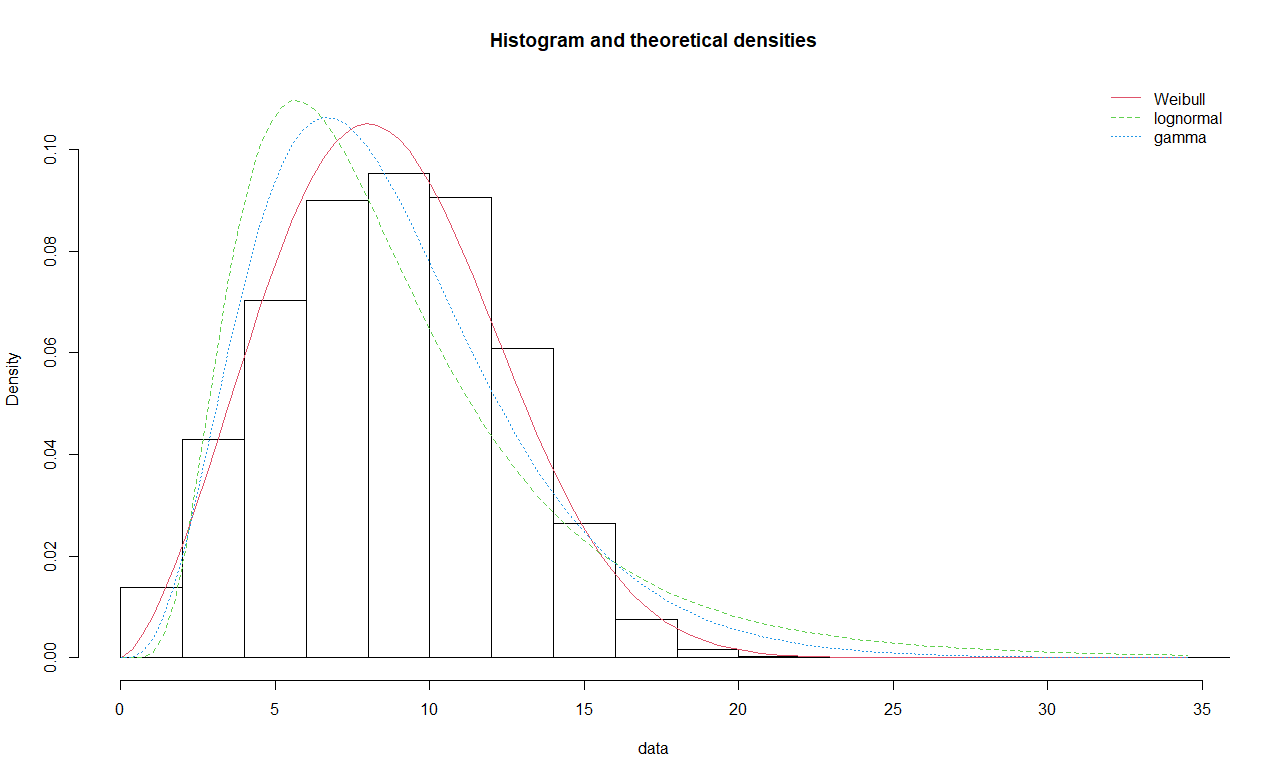
\includegraphics[width=0.45\textwidth]{figures/5yearcomparisonspeed}
    \caption{Histogram and Theoretical Densities, 5 year wind speed distribution}
    \label{fig:comp1}
  \end{figure}

  \begin{figure}
    \centering
    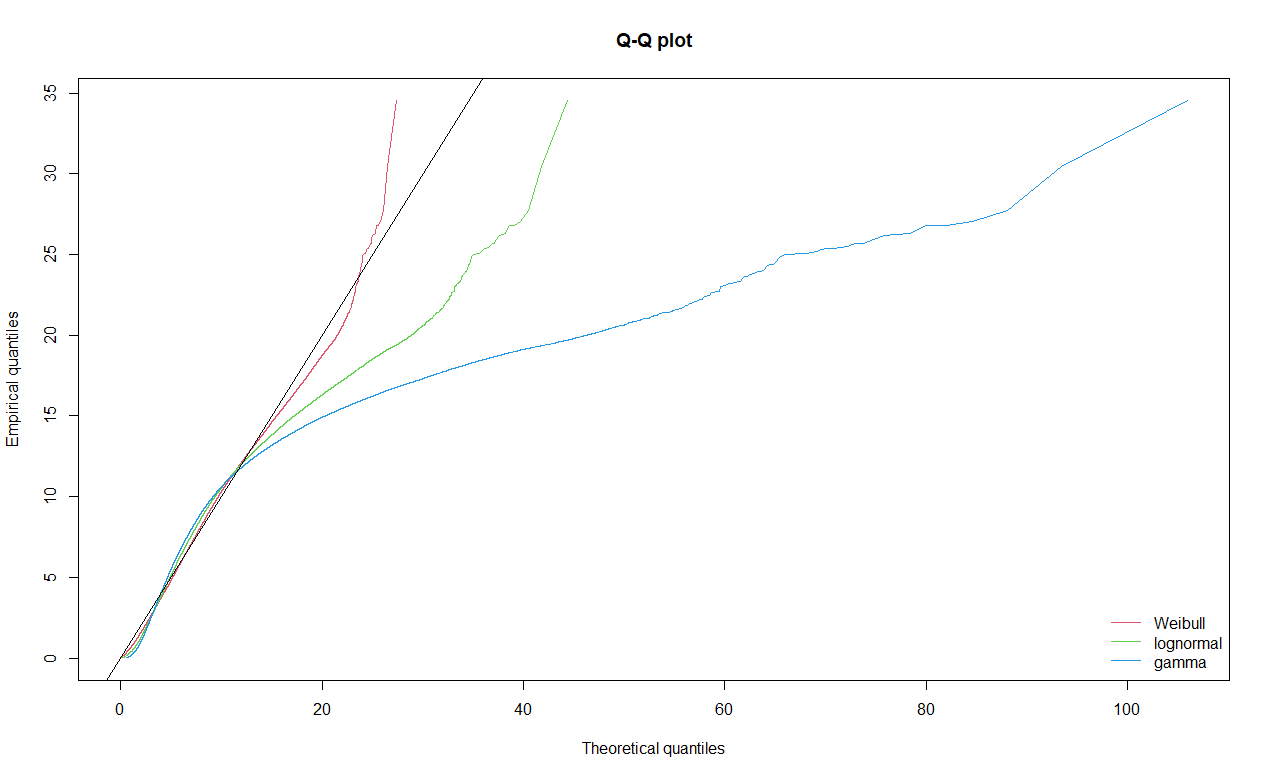
\includegraphics[width=0.45\textwidth]{figures/QQ5year}
    \caption{QQ Plot - 5 year wind speed distribution}
    \label{fig:comp2}
  \end{figure}

  \subsubsection{Goodness of Fit Criteria - Wind Speed}

  The Kolmogorov-Smirnov (KS) test is a numeric measurement of how closely the fitted distributions approximate the empirical data. This paper uses the KS test to determine the best fitted distribution for both wind speed and wind power. The lower the value is on the KS test, the better the fit. Table \ref{tab:distributions} shows the results of the KS test for wind speed. We can see that for wind speed, the Weibull distribution is the best fit for each year, and the 5 year total.

  \begin{table}
    \centering
    \caption{Goodness of Fit - Wind Speed Distribution Fitting}
    \begin{tabular}{c c c c}
      Distribution Type & Weibull & Log Normal & Gamma \\
      \hline
      2008 & 0.03430183 & 0.09372585 & 0.06096542 \\
      2009 & 0.02827901 & 0.08798708 & 0.06110601 \\
      2010 & 0.03430183 & 0.10437142 & 0.07339146 \\
      2011 & 0.03785982 & 0.09587753 & 0.0718786 \\
      2012 & 0.03649529 & 0.09845578 & 0.06939974 \\
      5 Years & 0.03143251 & 0.09576451 & 0.06697138
    \end{tabular}
    \label{tab:distributions}

  \end{table}

  \subsection{Wind Power}

  For the wind power, we will be using a Gaussian Mixture Model. A Gaussian Mixture is a function that is comprised of several Gaussians identified by $ k \in \{1, \ldots, K\}, $ where $ K $ is the number of clusters in our dataset \cite{carrasco_2020}. A cluster refers to a collection of data points aggregated together because of certain similarities \cite{carrasco_2020}. Each Gaussian has a mean $ \mu $ that defines its center, a covariance $ \Sigma $ that defines its width, and a mixing probability $ \pi $ that defines how big or small the gaussian function will be \cite{carrasco_2020}. Higher dimensional Gaussians are fully specified by a mean vector and a d by d covariance matrix \cite{ethen}.

  For our purposes, we can see that the wind power data can be grouped into at least two clusters. One for when the site is generating power and one for when the site is not generating power. However, in order to determine the best fit, we will be comparing different amounts of clusters and covariance types with the Bayesian Information Criterion (BIC). We will test the fit of 2 clusters to 4 clusters, along with different covariance matrix formulations which we will get into in the next section.

  \subsubsection{Goodness of Fit Criteria - Wind Power}

  The BIC is a criterion for model selection among a finite set of models \cite{BIC}. The model with the lowest BIC is preferred \cite{BIC}. The BIC is closely related to the Akaike Information Criterion \cite{BIC}.

  \subsection{GMM Fitting}

  The Scikit-Learn library contains a function that fits a GMM to a set of data given the number of clusters and covariance type. There are four covariance types.

  \begin{enumerate}
    \item full - each component has its own general covariance matrix
    \item tied - all components share the same general covariance matrix
    \item diag - each component has its own diagonal covariance matrix
    \item spherical - each component has its own single variance
  \end{enumerate}

  Because our data is univariate, the full, diag, and spherical formulations will score very closely to each other. In fact, the model scores are so close python has trouble differentiating due to floating point math inaccuracies. Fig. \ref{fig:GMM1} shows the BIC score per model. Each covariance formulation is tested along with the number of clusters. Below the BIC scores is the winning GMM model. The lowest BIC score in this test was 4 clusters with the spherical formulation. Fig. \ref{fig:GMM2} shows a close up view of the BIC scores for 4 clusters.

  \begin{figure}
    \centering
    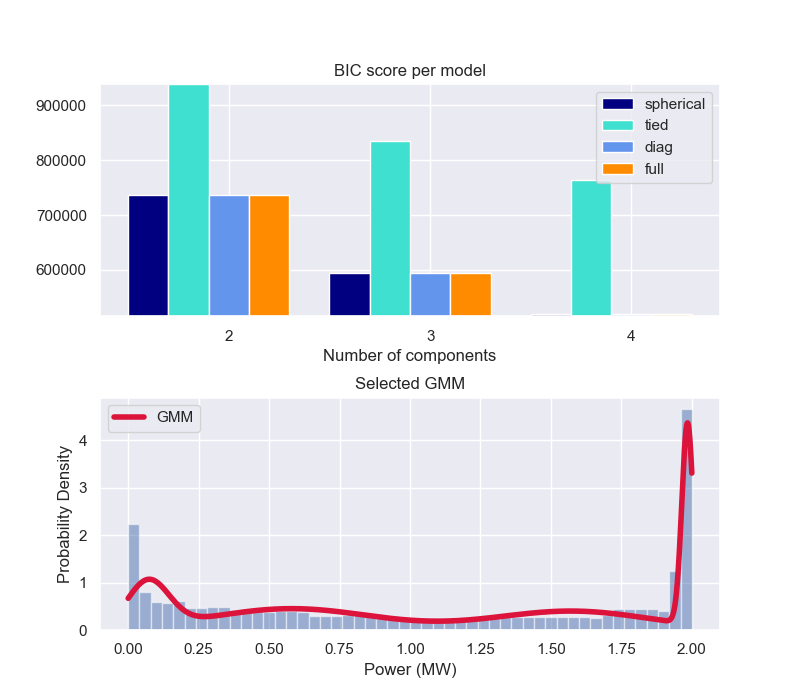
\includegraphics[width=0.45\textwidth]{figures/GMMdecision}
    \caption{Top Panel: BIC Scores for number of clusters and formulation. Bottom Panel: Winning GMM model plotted against 5 year wind power data}
    \label{fig:GMM1}
  \end{figure}

  \begin{figure}
    \centering
    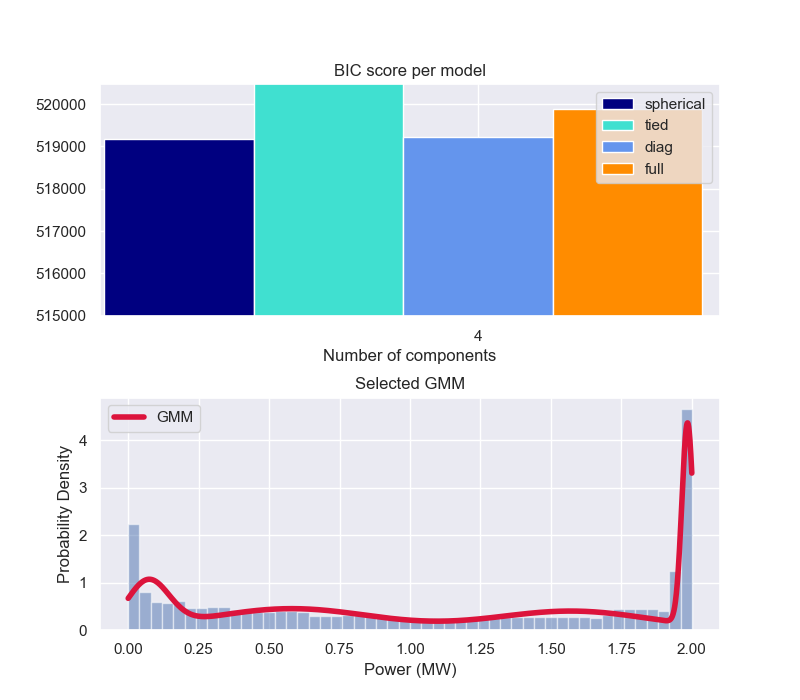
\includegraphics[width=0.45\textwidth]{figures/GMMdecision2}
    \caption{Close up of BIC scores for 4 cluster tests}
    \label{fig:GMM2}
  \end{figure}

  \newpage

  \section{Conclusion}

  A time series analysis of wind speed and wind power data was preformed. The seasonal trends for one week of wind speed and wind data were analyzed along with the 30 day rolling average for year long wind speed and wind power data. The relationship and correlation between wind speed and wind power was also discussed.

  Additionally, theoretical distributions were fitted to the wind speed and wind power data. The best fit for the wind speed data was determined using the KS test. The wind power data was fitted using GMM. Different amounts of clusters and covariance matrix formulations were tested and the best model was chosen using BIC scores.

  \bibliographystyle{ieeetran}
  \bibliography{References}



\end{document}
